\subsection{Client Design}

When designing the client we first looked through the requirements (listed in
Section \ref{sec:requirements}) to decide which features would need to be
developed in the client. Most features had root in the server but required a
layer in the client as well, and a few were to be developed in the client only.
A few requirements were not implemented in the service, and were hence dropped
for the client (see Section \ref{sec:futureimps}).

Requirement 25, which details that managers should have access to
all movies and songs for free, is implemented mostly in the client. If the user
that is logged into the system is a manager, the buy and rent button are hidden,
and the buttons for downloading or watching the material are shown instead. There
is some validation in the web service, but the majority of the implementation lies
in the client.

After prioritizing the list of features, we developed it into a list of views,
each view representing something a user of the client would see (see Appendix
\ref{app:client-views}). Each feature was not necessarily exactly one view (most
views contained several features).

For example, \emph{Manager overview} view were to provide "functionality
for uploading/creating new movies and songs", covering requirements 26 to 28.

We then implemented the views, feature by feature. This means that some views
were first developed in an \emph{incomplete} state, with the most highly
prioritized feature, and then later developed into the full planned view.

\subsubsection{Choice of technology}

As is common in web development we have used HTML\footnote{Hypertext Markup Language,
which is the standard language used to describe website content.} to mark up the
structure of the client, CSS\footnote{Cascading StyleSheets, the standard language
used to style website content.} to handle the styling/displaying of the website and
Javascript for the behavior of the website (event listeners etc.).

Besides these standard web technologies, we have supplemented
our Javascript with the JQuery framework, which provides facilities for
DOM\footnote{Document Object Model, a model of the objects in a web-page, described in
HTML, but accessible from Javascript.} manipulation and cross-browser compability of
event listeners. We have also made use of various JQuery plugins e.g. for cookie handling.
Using the JQuery framework made our development faster, as it provides shorthand functions for the most commonly used javascript features. The availability of these shorthand functions, meant that we could write in one line, what would otherwise take up several lines of code.

With our client we wanted to show that our web service allows for a simple \emph{server-free}
client solution and as such we have chosen to avoid server side coding completely in the
client solution although our group has extensive experience in server side scripting. This
choice allowed us to avoid a degree of indirection in our product, since every request goes
directly from our Javascript to the web service instead of going to a server-side script
first. This leads to an increase in the performance of our client (elaborated below), as well as a decrease in the load on the client's server, since every script is run locally in the user's browser.

We communicate with the web service through a technology called AJAX\footnote{Asynchronous
JavaScript and XML, which enables data to be sent from a server to a webpage. The data is
not limited to the XML format, and may also be in (for example) JSON.}, which enables us to
retrieve JSON\footnote{JavaScript Object Notation, a light-weight data format, which mimicks
the format of objects in the Javascript language.} data from the web service asynchronously.
Besides fetching the web service data through AJAX, we also use the technology whenever the
user wants to navigate to another page in the client. This has a lot of impact on the performance of our client as we are able to fetch the 
main part of the page asynchronously, while never actually reloading the whole page. Since we never have to reload the whole page, we only have to initialize our client once (setting up the navigation bar, JavaScript variables, and general frameworks), which gives us faster page loads and, as a result, a better user experience.

We have created a simple framework in Javascript, which provides the functions for navigation and the initialization of our global javascript variables. An example use of the framework is shown in Figure \ref{fig:ajax}.

\begin{figure}[hbt]
	\centering
	\centerline{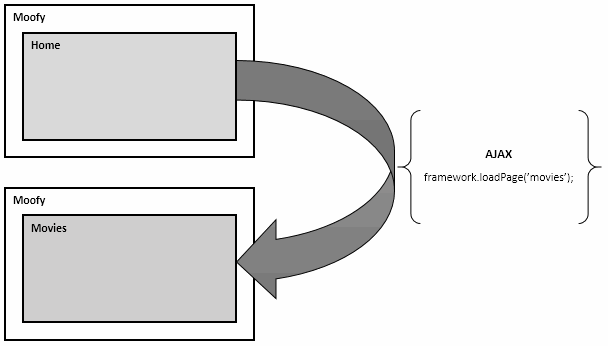
\includegraphics[scale=0.7]{./p1design/ajax.png}}
	\caption{Example of asynchronous page navigation through our framework.}
	\label{fig:ajax}
\end{figure}

The styled visual appearance of our client can largely be attributed to the use of the front-end framework Twitter Bootstrap, which provides the CSS styling of our navigation bars, forms, icons, buttons, etc. We chose this framework, since it allowed us to skip about a lot of manual css styling, and increased the speed of our prototyping. As a supplement to Twitter Bootstrap we have created a JavaScript framework for outputting CSS-styled information to the user, either through success messages, error messages, or variations of modal dialog windows. This framework was used to speed up our own production speed as well as provide a consitent look and feel across the client.

A last note regarding the visual appearance of the client is the use of Gravatar\footnote{Globally Recognized Avatar, \emph{avatar as a service}, provides users with cross-site avatars tied to their email.}, which allows Gravatar users to have their profile picture shown in our client based on their email adress. We implemented this to show that the functionality of our service can easily be combined or extended in a client through the use of external services on the web.